\chapter[Problem Analysis]{Problem Analysis} % Main chapter title

\label{ChapterProblemAnalysis} % For referencing the chapter elsewhere, use \ref{Chapter1} 

This chapter focuses on analysing the problem domain, including details of an initial survey conducted prior to the system's implementation regarding its potential feature set, and information about the two key hardware aspects of the system; the target `\textit{e-puck}' robot platform, and the tracking camera. The chapter finishes with details of the software development tools used during the project, and explains the reasoning behind their choice over a number of other, similar tools.

%----------------------------------------------------------------------------------------

\section{Initial User Survey} \label{InitialUserSurvey}

A survey was carried out within the YRL in order to determine how best to implement the system, and to ensure that the system would be useful in practice once finished. The respondents were all actively engaged in robotics work, either in a research capacity or as a technician, and had experience and understanding of swarm robotics specifically. The survey aimed to determine if a level of interest existed for the proposed system, and then ascertain which specific features were most desired. This would go on to influence design choices and inform priorities during development.

%----------------------------------------------------------------------------------------

\subsection{Questions and Response Data}
\noindent\textbf{Question 1: Do you believe that a system for displaying internal robot data for a swarm of robots in real time would be useful when debugging swarm robotics behaviours and/or conducting swarm robotics experiments?}

\begin{longtable}{ l c c }
 \textbf{Answer} & \textbf{Votes} & \textbf{Percentage} \\ 
 \hline
 Yes & 4 & 80 \\ 
 No & 1 & 20 \\
 No Opinion & 0 & 0 \\
 \bottomrule
 \caption{Responses to Question 1.}
 \label{tab:QuestionOneData}
\end{longtable}

\clearpage
\noindent\textbf{Question 2: Do you believe that such a system would benefit from the inclusion of an 'augmented reality' component - whereby data retrieved from the robots could be displayed in graphical forms, overlaid on a live video feed of the robots themselves?}

\begin{longtable}{ l c c }
 \textbf{Answer} & \textbf{Votes} & \textbf{Percentage} \\ 
 \hline
 Yes & 5 & 100 \\ 
 No & 0 & 0 \\
 No Opinion & 0 & 0 \\
 \bottomrule
 \caption{Responses to Question 2.}
 \label{tab:QuestionTwoData}
\end{longtable}

\noindent\textbf{Question 3: Please rate each of the following potential features based on your opinion of their importance or usefulness to the system proposed, on a scale of one to five, where one indicates a feature is not important or useful, and five indicates a feature is very important or useful.}

\begin{figure}[h]
	\centering
	\makebox[\textwidth][c]{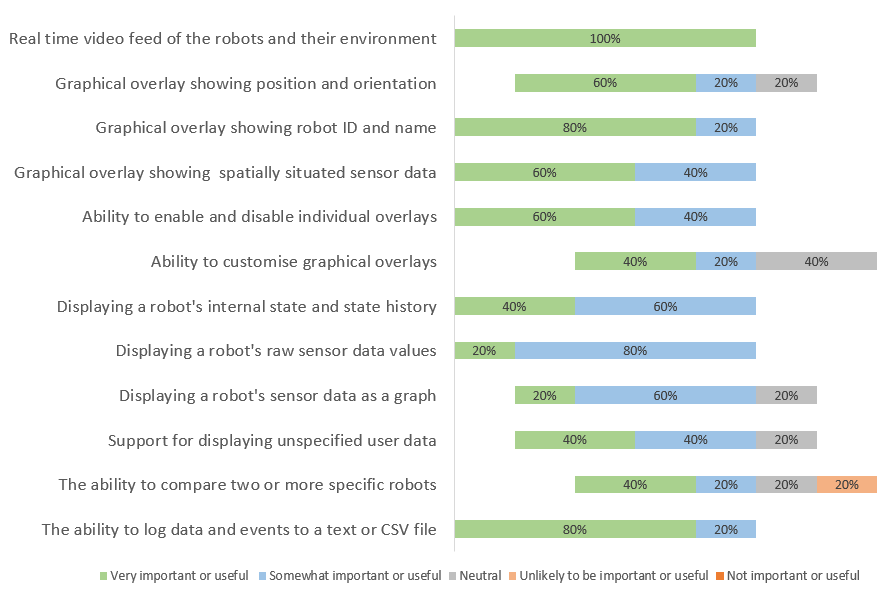
\includegraphics[width=1.1\textwidth]{FeatureLikert.png}}
	\decoRule
	\caption[Initial Survey Question 3 Results]{The results of Question 3.}
	\label{fig:FeatureLikert}
\end{figure}

%On the questionnaire the values of one to five were qualified as `\textit{Not important or useful}', `\textit{Unlikely to be important or useful}', `\textit{Neutral}', `\textit{Somewhat important or useful}' and `\textit{Very important or useful}' respectively.

%\begin{center}
%\begin{tabular}{ p{10cm} c c c c c }
% \textbf{Feature} & \textbf{1} & \textbf{2} & \textbf{3} & \textbf{4} & \textbf{5} \\ 
% \hline
% Real time video feed of the robots and their environment & 0 & 0 & 0 & 0 & 5\\
% Augmentation of the video feed with the position and orientation of each robot & 0 & 0 & 1 & 1 & 3\\
% Augmentation of the video feed with each robots identifier (ID or name) & 0 & 0 & 0 & 1 & 4\\
% Augmentation of the video feed with spatially situated sensor data, represented in a graphical form & 0 & 0 & 0 & 2 & 3\\
% The ability to enable and disable individual elements of the video feed augmentation & 0 & 0 & 0 & 2 & 3\\
% The ability to customise individual elements of the video feed augmentation (colour, size, etc.) & 0 & 0 & 2 & 1 & 2\\
% Displaying the robots internal state and a history of recent state transitions & 0 & 0 & 0 & 3 & 2\\
% Displaying raw sensor data (e.g. IR) in textual format & 0 & 0 & 0 & 4 & 1\\
% Displaying sensor data in plotted graph formats & 0 & 0 & 1 & 3 & 1\\
% Support for displaying unspecified user data in textual form & 0 & 0 & 1 & 2 & 2\\
% The ability to compare two or more specific robots within the swarm & 0 & 1 & 1 & 1 & 2\\
% Logging received data and events to a text or CSV file & 0 & 0 & 0 & 1 & 4\\
%\end{tabular}
%\end{center}

\clearpage
\noindent\textbf{Question 4: Please briefly describe any additional features you believe would be useful, based on your experiences working with swarm robotics systems.}

\begin{itemize}
\item ``\textit{macro-level behavioural data on the swarm; e.g., number of robots in different behavioural states (color coded accordingly).}''
\item ``\textit{I think the system (already potentially very useful) could be improved/expanded further to add the option of more post-processing/extraction of data. The ability to create video of the over-lay, and perform statistical analysis on the complete run, would begin to turn the system in not only a very useful debugging system but a complete package allow researchers to gather high-quality, publication ready analysis of swarm experiments.}''
\end{itemize}

\noindent\textbf{Question 5: Which of the following aspects of the robot data do you believe should be made available by the application to aid in debugging and testing? Tick all that apply. Please add any more you may think of.}

\begin{longtable}{ p{10cm} c }
 \textbf{Data Type} & \textbf{Votes}\\ 
 \hline
 Position & 4\\
 Orientation / direction & 4\\
 Position change over time (recent path tracking) & 4\\
 Internal state machine state & 3\\
 Internal state transition history & 3\\
 IR sensor values & 4\\
 Distance between robots & 3\\
 Robot ID & 4\\
 Other & 2\\
 \bottomrule
 \caption{Responses to Question 5.}
 \label{tab:QuestionFiveData}
\end{longtable}

Additional responses:

\begin{itemize}
\item ``\textit{Option to include user-defined data so if a certain controller implements a timer that facilitates a state transition might be useful to see the value of that timer whilst debugging to compare with state transitions.}''
\item ``\textit{A simple API to add user-defined variables/statuses.}''
\end{itemize}

\noindent\textbf{Please add any additional comments you have about the proposed application in relation to your experiences working with swarm robotics systems.}

\begin{itemize}
\item ``\textit{A client-server model between back-end (camera) and remote client would potentially be very useful; also the system should be flexible and not reliant on a specific camera/server setup. Would be very interesting to see if it will work on a R-Pi 3 + camera combination, as this would allow for portable tracking setups.}''
\item ``\textit{All real-time information is useful!}''
\end{itemize}

%----------------------------------------------------------------------------------------

\subsection{Analysis}
The positive response to question one indicates a reasonable level of interest in the system amongst those surveyed. The similarly positive response to question two adds more weight to the idea that graphical debugging tools have the potential to be particularly useful in a robotics context, as established during the literature review. The responses to these two questions indicate that interest exists for the system, and that it is worthwhile implementing it. This satisfies the first aim of the survey.

The remainder of the survey focuses on establishing which features are most desirable, and the results were used when considering implementation priorities. The response to question three indicates that the majority of the core features were thought to be potentially useful, especially those related to the video feed and overlay. Tertiary features such as customising the colours and sizes of the overlays showed less interest. This was as expected, as these kinds of features do not aid directly in the debugging process. Considerable interest was expressed in the ability to log data and events, a feature which was not considered a major priority at the outset. Conversely, the ability to compare two robots was the only feature to receive a vote lower than neutral, despite being initially thought a key feature of the system. As a result the implementation of logging was moved up to a main priority, and the comparison feature was reduced to non-essential.

The respondents were then given the chance to optionally suggest additional features in question four. The first of the two responses suggests `macro-level behavioural data', a concept considered during the project's inception. It was not included in the initial plan or survey partly because at the outset it was not clear what form the feature would take, or whether it would be feasible in the time frame, and partly because it was seen as a feature related more to analysing swarm experiments and results rather than debugging. As a result of this answer displaying macro level swarm data was considered a desirable but not essential feature, to be implemented if time allowed. The second response offers a broader vision for the system as a whole. This report agrees with the observation of the system's potential to become a complete package for analysing swarm experiments and extracting data, however the majority of the features mentioned are considered beyond the scope of this project. This includes video extraction and post processing of data. The expansion of the system is discussed in chapter \ref{ChapterConclusion} where possible future work is discussed.

Question five attempts to establish which specific data types are most desirable in the system. Note that one respondent did not answer this question at all, leading to the lower vote counts. None of the data elements listed received a significant deficit in votes, suggesting that all the data types listed should be included. Respondents were asked to optionally suggest other data types, and the two responses received both independently identified user-defined data or 'variables' as a desirable data  type. The inclusion of custom user defined data was a planned part of the system from the beginning, and is mentioned in question 3, but these responses confirmed that it should be a priority feature of the system.

The final section gave respondents the opportunity to add any additional comments about the system. The first response notes that designing the system in a way which does not make it `reliant on a specific camera/server setup' would improve its usability. This thinking matches the stated objective of making the system in a modular way that is easily extensible with different camera set-ups and different robots.

%----------------------------------------------------------------------------------------

\subsection{Issues and Shortcomings}
This survey provided a useful tool for gaining a general impression of relevant opinions regarding the project and the system. However it also had a number of issues in its execution which might somewhat diminish the value of the data. Firstly due to the highly specific nature of the desired participants, the sample size is extremely small. Care must therefore be taken in analysing the results too deeply; for example any statistical analysis performed would likely be flawed. Another issue is that the two larger multiple choice questions present a relatively small selection of possible features and data types, based on those already planned or considered for implementation.  This report therefore aims to use the results in an indicative, holistic manner to guide implementation, rather than quantitatively define the feature set.

%----------------------------------------------------------------------------------------

\section{Hardware - E-Puck Robot Platform}
The e-puck robotic platform, created by a team at the \textit{Ecole Polytechnique Fédérale de Lausanne} \cite{epuck}, is a small, relatively inexpensive, multi-purpose robotic platform designed for education and research pursuits in robotics and multi-robot systems. The platform is widely used in swarm robotics research, featuring in a number of publications. The e-puck was chosen as the first target platform for this system for a number of reasons. Firstly this was one of the platforms available in suitable numbers in the YRL, where the practical work for this project was carried out. Secondly the platform's wide use in swarm robotics research helps to show the broad applicability of the system, and better demonstrates its value when compared to a less widely used or bespoke platform. Finally the platform's extensible design meant that it could be equipped with an extension board featuring an ARM9 processor running a Linux operating system, a configuration frequently used at the YRL. This enabled the use of WiFi for wireless data transfer, and was a large part of the reasoning behind choosing the e-puck. This section provides details of the e-puck robot's hardware, including its processor, sensors and actuators, as well as details of the Linux extension board. Figure \ref{fig:EPuck} shows the e-puck robot, equipped with the Linux extension board on top.

\begin{figure}
	\begin{center}
	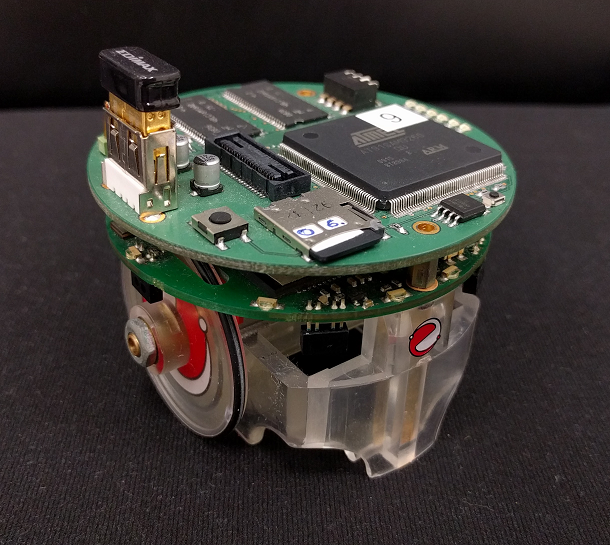
\includegraphics[scale=0.6]{EPuck.png}
	\decoRule
	\caption[The e-puck Robot]{The e-puck robot, equipped with a Linux extension board.}
	\label{fig:EPuck}
	\end{center}
\end{figure}

%----------------------------------------------------------------------------------------

\subsection{Processor}
The e-puck features a \textit{dsPIC 30F6014A} microprocessor, designed and manufactured by Microchip Technology Inc. This is a general purpose 16-bit CPU, with relatively low performance by modern standards. The processor features 68 I/O pins, which are connected to the e-puck's various peripherals. Due to the use of the Linux extension board discussed in section \ref{LinuxExtensionBoard}, which features a more powerful ARM processor, the primary use of the PIC processor in this configuration is to interface with the e-puck's hardware. This involves receiving commands from the ARM processor and sending appropriate control signals to the robot's actuators, as well as reading the robot's sensors and passing the retrieved sensor data back to the ARM processor. Prior to the start of this project members of the YRL had already developed a library of low level code allowing the PIC to function in the hardware interface role described, controlled through a UART serial connection. This firmware code was used as-is on the e-pucks' PIC processors throughout the project.

%----------------------------------------------------------------------------------------

\subsection{Actuators}
The e-puck robot features two wheels, independently actuated by two step motors. The wheels have a diameter of approximately 41mm. The motors can rotate the wheels at an approximate maximum speed of 1000 steps per second in either direction, where 1000 steps is one full revolution. The robot also features a ring of 8 red LEDs around the edge of the main circuit board, which can be controlled for any arbitrary purpose. 

%----------------------------------------------------------------------------------------

\subsection{Sensors}

\begin{figure}
	\begin{center}
	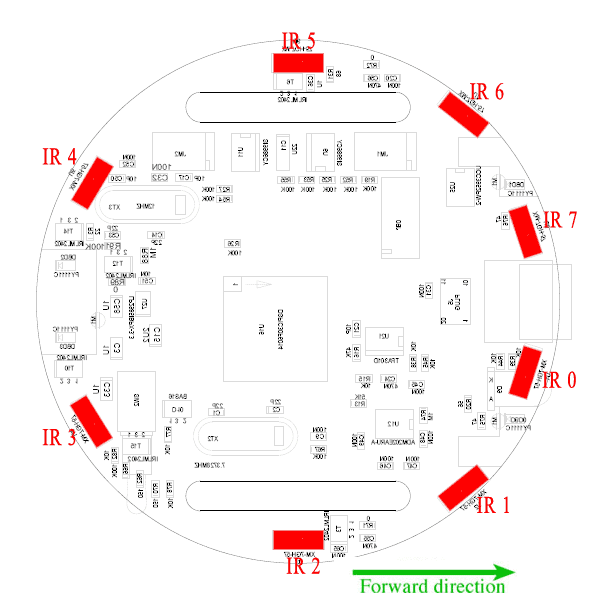
\includegraphics[scale=0.4]{EPuckIRSensors.png}
	\decoRule
	\caption[E-puck IR Sensor Layout]{The layout of the IR sensors on the e-puck robot.}
	\label{fig:EPuckIRSensors}
	\end{center}
\end{figure}

The e-puck robot features a number of different sensor sets, of which only some are used in this project. A set of 8 IR proximity sensors are arranged around the circumference of the robot, with four positioned on the forward hemisphere, two positioned at right angles to the forward direction (one on either side) and two more positioned on the backward hemisphere at roughly 45 degrees either side of the backward direction. Figure \ref{fig:EPuckIRSensors} shows this layout. The IR sensors can be used in two modes - active and passive. In active mode the sensor emits an IR pulse and measures the strength of the reflection, whereas in passive mode the sensor simply samples the IR strength without emitting a pulse. The passive mode can therefore be used to get a 'background' IR reading, which can be compared to the active reading to improve accuracy. The IR sensor is of particular interest to this project as it is a frequently used tool when working with robots, especially robot swarms. The robot also features three microphones, a 3 axis accelerometer and a camera. Due to the bandwidth required to use the microphones and camera they were considered a low priority for this project.

%----------------------------------------------------------------------------------------

\subsection{Linux Extension Board} \label{LinuxExtensionBoard}
For this project the e-pucks were fitted with an extension board featuring a 32-bit ARM9 processor running a modified Linux operating system \cite{LinuxExtensionBoard}, developed by Wenguo Liu, and Alan F.T. Winfield. In this configuration the ARM processor, an Atmel AT91, takes charge of the high level robot control logic, as well as any intensive data processing operations. The dsPIC processor is then used to control the low level actuator and sensor control, running in parallel with the ARM processor and communicating via UART. The extension board provides a USB port, and for this project a WiFi adapter was connected to each robot. The controller code running on each robot could then make use of the standard IP network layer protocol, and the standard transport protocols TCP and UDP.

%----------------------------------------------------------------------------------------

% (Chapter 6)

\section{Hardware - Video Tracking System} \label{TrackingHardware}

In order to implement the augmented reality element of the system, and satisfy the related objectives, a live video feed of the swarm was needed. A method for tracking the positions of each individual robot in the swarm within each video frame in this feed was also required, in order to correctly position the graphical overlays. Prior to the start of this project infrastructure had been put in place at the YRL for performing this kind of video-based tracking task, in the form of a machine vision camera placed above a robot '\textit{arena}'. Figure \ref{fig:CameraLayout} shows the arrangement of the machine vision camera and the robot arena. Figure \ref{fig:ArenaPhoto} shows a photo of this set up at the YRL. Ongoing research being carried out by members of the YRL has already made use of this camera and arena set up, in conjunction with image processing software for tracking fiducial markers within the image, to achieve robot tracking with good accuracy and relatively high frame-rate.

The image processing in these ongoing research efforts was performed using the `ArUco\cite{Garrido:2014}' fiducial marker based tracking system, discussed further in section \ref{ArUco}. It was determined that incorporating this existing infrastructure into the swarm debugging system would be the quickest way to achieve an operational tracking system, allowing work to focus on the novel aspects of the project sooner.

\begin{figure}
	\centering
	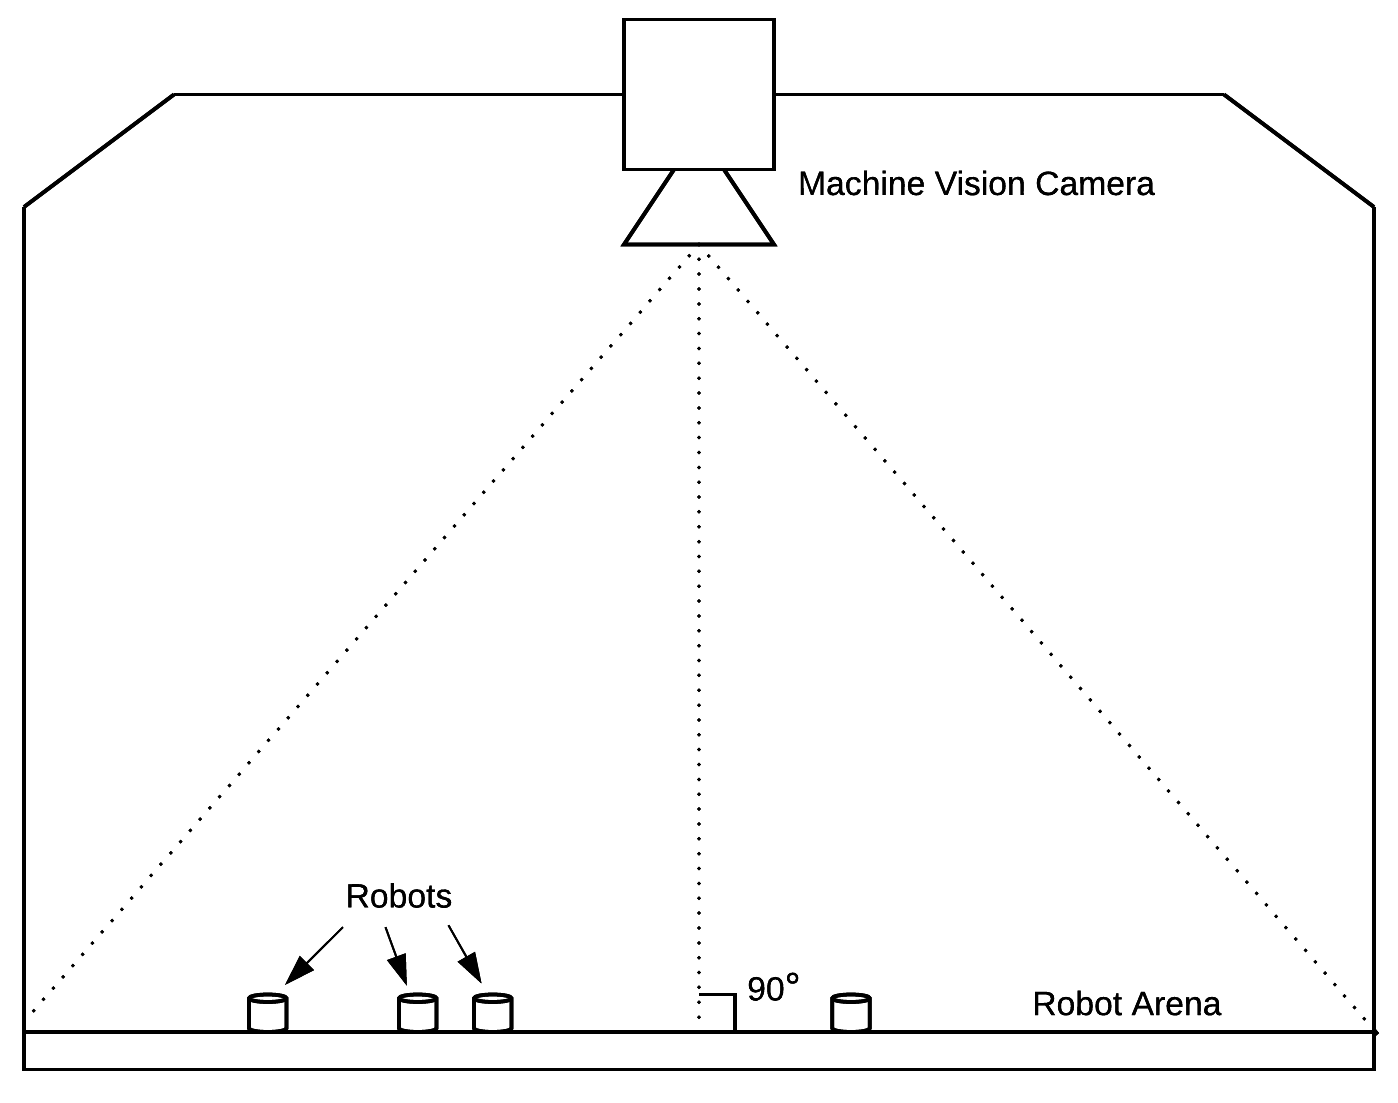
\includegraphics[scale=0.3]{Figures/CameraLayout.png}
	\decoRule
	\caption[Tracking Camera Arrangement]{Arrangement of the tracking camera over the robot arena.}
	\label{fig:CameraLayout}
\end{figure}

\begin{figure}
	\centering
	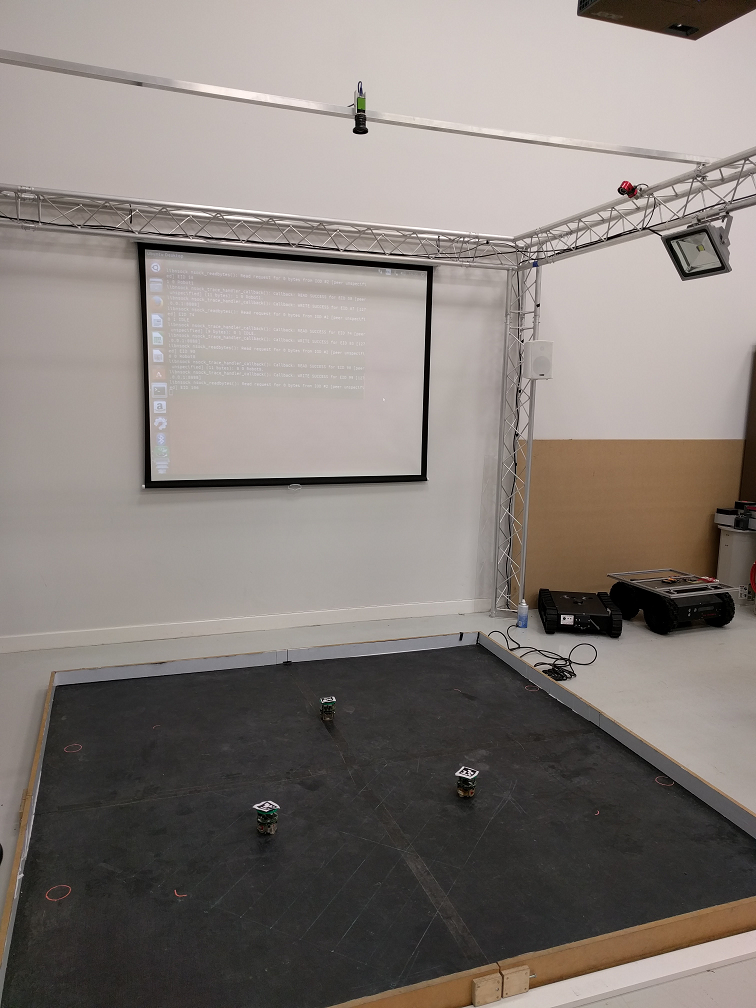
\includegraphics[scale=0.4]{Figures/ArenaPhoto.png}
	\decoRule
	\caption[Robot Arena and Tracking Camera]{The robot arena set up at the YRL, with tracking camera visible.}
	\label{fig:ArenaPhoto}
\end{figure}

%----------------------------------------------------------------------------------------

\subsection{Camera}
The camera used in the aforementioned tracking set-up is a JAI Go 5000C-PGE colour, area-scan camera, shown in figure \ref{fig:Camera}. It features a 1-inch, 5-megapixel CMOS sensor, with a maximum resolution of 2560 by 2048 pixels, capable of capturing 22 frames per second at full resolution, and up to 163.5 frames per second with reduced resolution and colour quality. The camera also features a global shutter, meaning it captures the full area of the image simultaneously, as opposed to a rolling shutter which captures portions of the image sequentially. This camera is well suited to marker tracking applications for a number of reasons. The high resolution means that even small markers, or markers that are relatively far from the camera will be captured with sufficient detail to be tracked and identified. The relatively high frame-rate means that the tracked positions can be recalculated regularly, and the video will appear smooth. The use of a global shutter avoids issues present in rolling shutter cameras, where a moving marker appears broken due to the time difference between the capture of two areas of the image and the movement of the marker during this time.

\begin{figure}
	\centering
	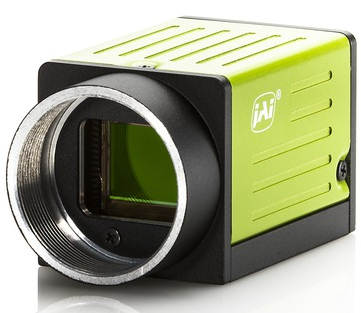
\includegraphics[scale=0.8]{Figures/Camera.png}
	\decoRule
	\caption[JAI-Go Camera]{The JAI-Go 5000C-PGE camera \cite{JAIGoCamera}.}
	\label{fig:Camera}
\end{figure}

The camera is connected to a server rack using Gigabit Ethernet cable, which is required to support the high bandwidth output of the camera due to its resolution and frame rate. This cable also provides power to the camera. A high resolution lens is fitted, with a relatively wide range of possible focal ratios from $f/1.4$ to $f/16$, allowing the camera to be adjusted to work well in a range of light conditions. With the lens included the camera has approximate dimensions of $29 \times 29 \times 100$ mm, and a weight of 246 grams, making it a very compact, lightweight solution.

The image data from the camera is transmitted in accordance with the `\textit{GigE Vision}' interface standard \cite{GigEVision}. This standard was first introduced in 2006, and is designed for transmitting video from high-performance industrial cameras over Ethernet networks. The `Common Vision Blox' (CVB) machine vision programming library is used to map the data from the GigE format to the OpenCV image format, so that it can be processed by an application.

%----------------------------------------------------------------------------------------

\subsection{ArUco Tracking System} \label{ArUco}
Developed by a team from the Computing and Numerical Analysis Department of Cordoba University in Spain, the ArUco tag generation and detection system \cite{Garrido:2014} is a powerful fiducial marker creation and tracking tool. It comprises an algorithm for producing a dictionary of square, black and white, coded markers, and further algorithms for automatically detecting these markers in a given image. These markers can be easily printed using a standard printer, and attached to surfaces and objects. Figure \ref{fig:ArUcoTags} shows four possible marker variations on standard printer paper. The stated applications for the ArUco system include augmented reality, machine vision, and robot localisation. One of the main benefits of this system over other fiducial marker systems is the execution speed. By first using edge-detection methods to isolate the outlines of potential markers in the image, the system can eliminate a large portion of the image before applying the more complex processing to identify and differentiate individual markers \cite{Garrido:2014}. This makes the algorithm extremely efficient, and therefore makes it possible for the ArUco system to be run in real time, even with relatively modest computational power. In a conventional use case the orientation of the camera can be calculated based on the positions of the corners of a marker, if the marker's orientation is known. In the use case of this project the reverse is true; the camera's position is fixed, and therefore the orientation of a robot can be determined based on the position and orientation of the corners of its marker.

\begin{figure}
	\centering
	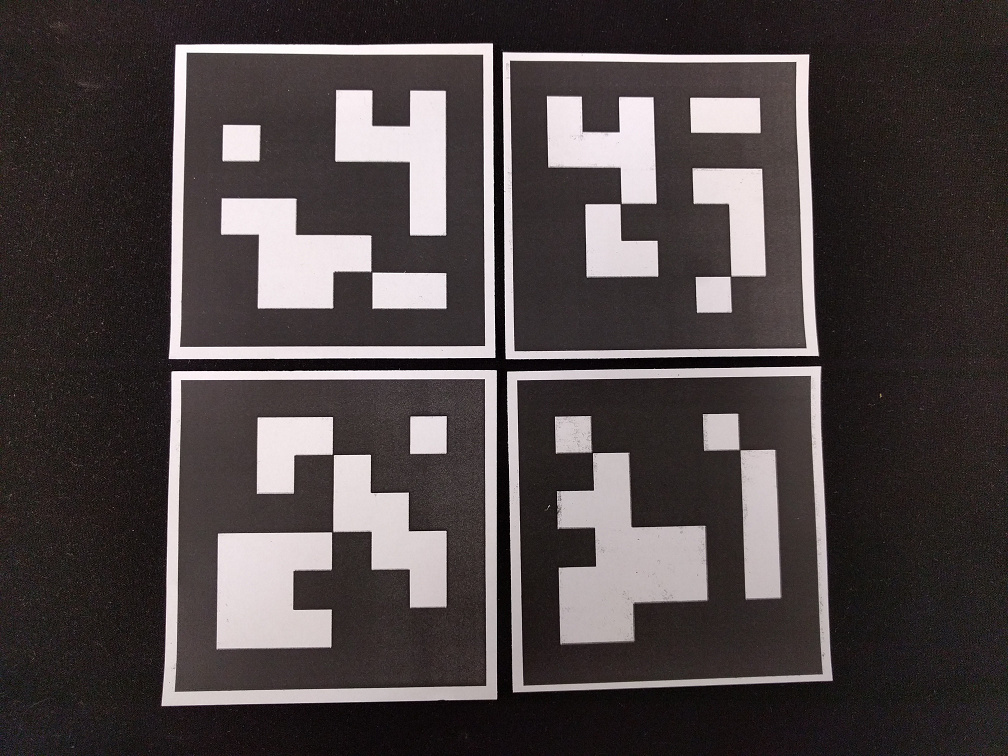
\includegraphics[scale=0.3]{Figures/ARuCoTags.png}
	\decoRule
	\caption[ArUco Markers]{Four markers generated by the ArUco fiducial marker generation and detection system, and printed using a standard printer.}
	\label{fig:ArUcoTags}
\end{figure}

Each of the e-puck robots used in this project were assigned an ID number, and a dictionary of ArUco markers was generated to match. The markers were affixed to the top of the robots, oriented to match their forward directions. Figure \ref{fig:EPuckArUco} shows a laser printed ArUco marker mounted on top of an e-puck robot. Some cursory preliminary tests of the tracking system confirmed that the markers could be accurately and reliably detected in the camera images, at a decent frame rate. Further detail of the integration of the ArUco marker tracking system into the application developed during this project is given in section \ref{VideoFeedAndTrackingSystem}.

\begin{figure}
	\centering
	\includegraphics[scale=0.5]{Figures/EPuckARuCo.png}
	\decoRule
	\caption[ArUco Marker Mounted on e-puck]{A laser printed ArUco marker mounted on top of an e-puck robot.}
	\label{fig:EPuckArUco}
\end{figure}

%----------------------------------------------------------------------------------------

\section{Software Development Tools} \label{SoftwareDevelopmentTools}

Throughout the implementation process a number of tools were used to enable and organise development. Software development is a tool-rich field, and selecting the right tools, and using them effectively, can result in significant increases in development efficiency. 

\subsection{\textit{Git} Version Control System}
Version control is an important concept in software development \cite{VersionControl}, and a variety of tools exist to help developers manage the process. The purpose of a version control system (VCS) is to handle additions and changes to a code-base in an organised, structured fashion, such that each new change is logged, and can be reversed if necessary. This means that if some feature or functionality is broken by a change, it is trivially easy to revert the code-base to its state before the change in order to recover the functionality. It also helps with debugging by allowing a developer to examine the specific contents of a change that has caused a problem, without relying on memory. Version control also enables multiple developers to work on the same code-base simultaneously \cite{SVCPatent}, as it automatically checks for collisions between new changes. Most version control systems are based around a code `\textit{repository}', which stores the code, as well as information regarding every change made. In a standard distributed model developers download a copy (or `\textit{clone)'} of the code from this repository to their development machine. Details of changes made to their local copy are stored in `\textit{commits}', which allows the developer to add a message to describe each change. These commits can then be uploaded (or `\textit{pushed}') to the main repository. These repositories are usually hosted online or on a private server, allowing developers to work in a distributed fashion, and removing the risk of significant code loss if one development machine is lost for any reason.

For this project the \textit{Git} version control system \cite{ProGit} was chosen, in conjunction with the \textit{Github} repository hosting service \cite{Github}. Github is a widely used online software repository hosting service which supports all of the functionality of the Git VCS, as well as a number of other convenience features including analytical and project management tools. Github and Git were chosen for this project for several reasons. Firstly, both are widely known and used in the software development world, suggesting reliable and well developed functionality. This combination is also regularly used within the YRL for other software development. The Github service is also free to use, thus avoiding any cost to the project. Finally previous experience with both the Git VCS and the Github repository hosting service had been positive, and suggested they would be suitable for this project.

A wide variety of VCSs exist, and a number were considered for use in this project. `\textit{Subversion}', commonly referred to as just `\textit{svn}', is another VCS with similarly widespread usage to Git \cite{Subversion}. However svn functions in a slightly different manner, requiring a connection to the server where the repository is hosted before any commits can be made. Git does not have this requirement, as commits can be made against the local copy of the repository, and later pushed to the main repository when a connection is available \cite{ProGit}, allowing the benefits of version control to be leveraged without a connection to the server. This was the primary reason Git was chosen over svn, as the development work for this project was to be completed on a laptop in a number of locations, without a guaranteed internet connection at all times.

`\textit{Mercurial}' \cite{Mercurial} is another VCS system with a similar feature set to Git. Like Git, Mercurial allows for commits against a local repository clone, removing the need for a constant server connection during development. For a project with development requirements as simple as this one, the slight differences between Git and Mercurial are unlikely to be relevant, hence the two were assessed to be essentially equivalent. It was therefore simply prior experience with Git, and the use of Git within the YRL, that led to its choice over Mercurial.

Similarly to VCSs, there are many repository hosting services available today, all with relatively similar feature sets and minor differentiating factors. `\textit{Bitbucket}' is another widley used, free, repository hosting service which supports the Git VCS. The service supports virtually all of the same features as Github, and would have been an equally suitable choice for this project. It was not chosen primarily due to the prevalent use of Github within the YRL, and due to prior experience with Github meaning less of a learning curve and therefore a shorter start up time for the project. Similarly other repository hosting services were ruled out based on the convenience of Github due to prior use. Another relevant factor was cost, as a number of other similar services, such as `\textit{Kiln}', require a paid subscription.

This was a single developer project, and therefore many of Git's team-based features were not necessary, and the tool was used simply for code storage and version control. Development was carried out on a single development branch, as there was no need to maintain a stable release branch, and no benefit to multiple feature branches given the lack of multiple developers. Once development was completed at the end of the project, the development branch was merged back on to the main branch, marking the completion of the first version of the software.

\subsection{\textit{QCreator} Integrated Development Environment}
An integrated development environment (IDE) is a software tool used when developing other software, providing basic functionalities such as text editing and file browsing, as well as specific features to help with development, such as syntax highlighting, error checking, build configuration management, built-in compiling, and debugging tools. IDEs are extremely useful tools when developing any piece of software that is non-trivial in size or scope, or has significant dependencies, and serve to accelerate work-flow and minimise issues.

Section \ref{ApplicationFrameworkSelection} discusses the choice of the \textit{Qt} application programming framework for implementing the swarm debugging application within this project. \textit{Qt Creator} \cite{QTCreator} is an IDE specifically designed to aid in the development of software applications based on the Qt application framework, making it the obvious choice for use in this project. Qt Creator offers a number of features to specifically support the Qt framework, including a graphical interface layout designer tool, which was used to compose the graphical interface for the application, and produced the \textit{mainwindow.ui} XML-like file which describes the application's UI layout. The IDE also provides integrated support for the \textit{QMake} build management system, which describes the files necessary to compile and build the application. The application could be compiled and run from within the IDE, which also features a debugger and supports standard tools such as breakpoints. The debugger was used regularly during development to locate issues and refine the implementation of features.

A number of other IDEs were considered for use during application development, including several which are more widely used and feature-rich than Qt Creator. `CLion' \cite{CLion}, a modern, feature rich IDE designed for C and C++ development was considered due to its powerful code analysis and suggestion feature set, cross platform support, and free student license. However ultimately it was determined that the benefits of Qt Creator's built-in support for Qt applications outweighed the benefit of CLion's superior feature set. CLion was considered again when choosing a tool for writing code to be run on the robots, separate from the main application code, however it quickly became apparent that, due to the relatively simple nature and scope of this portion of the code, the features of a full IDE would not be necessary. The `\textit{Sublime Text}' text editor \cite{SublimeText} was chosen instead, as this simple tool required minimal set up, but still supported useful development features including syntax highlighting.

%----------------------------------------------------------------------------------------

\section{Summary}
In this chapter analyses of a number of topics relevant to the project were presented. An initial user survey, carried out prior to the design and implementation of the system, was described and the results presented and discussed. This survey sought responses from potential users of the system, and in general showed an appetite for the system and many of its core features, but highlighted some planned features as less relevant than originally thought. Relevant infrastructure within the YRL was discussed, including the \textit{e-puck} robotic platform, which was the initial target platform for the system, as well as the camera hardware configuration, and the \textit{ArUco} tracking system. Finally the choices of software development tools were discussed, explaining the choice of \textit{Git} and \textit{Github} for version control and code repository hosting, and the \textit{Qt Creator} IDE and \textit{Sublime Text} text editor for code editing and development work. These analyses led to a better understanding of the problem domain, and allowed for the system to be designed and implemented effectively.